\chapter{Information-Theoretic Map Compression}
\label{chapter3}

The remaining chapters of this thesis introduce novel extensions to active perception
that make information-theoretic reward evaluation more
efficient at the cost of information-theoretic reward accuracy.
These extensions originate from the observation that the information content
of a robot's sensor measurement depends on the environment
representation. In the case of OG maps, the cell resolution parameter shares an
intricate relationship with the robot's exploration behaviors.

One example of the relationship between OG cell resolution and exploration
behavior lies in the efficiency of raycasting. Most information-theoretic reward
functions (e.g. SMI and CSQMI) require simulating a beam-based sensor measurement from a future
position, which implicitly requires raycasting through the map. Intuitively, as
the resolution of cells in the map decreases, so too does the number of cells
that a raycast must traverse. Therefore the efficiency of information-theoretic reward evaluation
is a function of the cell resolution of the OG. For example, using the approximate
CSQMI technique from Charrow et al.~\cite{charrow2015icra}, this relationship is linear
(Fig.~\ref{fig:csqmi_timing}). As will be shown, the resolution of an OG map can typically be halved several
times before a significant amount of information about free and occupied space
is lost. Repeatedly halving the map's resolution exponentially increases the
speed of computing CSQMI for a fixed sensor range or number of beams. This
can be seen by holding range constant and tracing vertical lines down Fig.~\ref{fig:csqmi_timing}.

The following chapter investigates map compression as a means of increasing the
efficiency of evaluating CSQMI reward. The incentive for increasing the efficiency of information-theoretic exploration
is clear and immediate; any reduction to the time required to evaluate an
information-theoretic reward function will enable a robot to explore more
efficiently, in turn allowing it to initialize faster (Fig.~\ref{fig:motivation}), clear a
building for threats more quickly, or explore a larger amount of space on an energy budget.


\begin{figure}
  \centering
  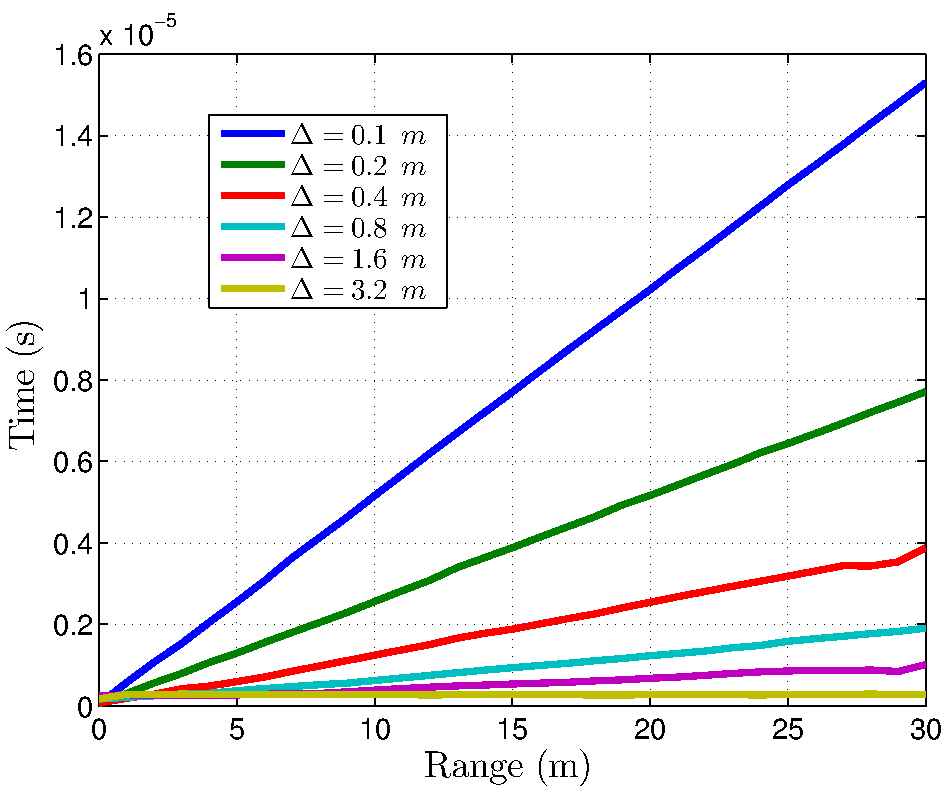
\includegraphics[width=0.65\textwidth]{csqmi_timing.pdf}
  \caption[Time complexity of computing CSQMI for a varying map resolution.]{Time (median of $10^5$ samples)
    to evaluate CSQMI for a single beam is empirically linear in both the OG
    cell edge length $\Delta$, and
  the measurement range. \label{fig:csqmi_timing}}
\end{figure}

Several others have proposed strategies for map compression. The OctoMap
framework~\cite{wurm2010octomap} builds an octree data structure to efficiently store the
expected occupancy of cells in an environment without allocating memory for a
large 3D grid. Jeong et al.~\cite{im2010real} compress an OG by representing it with
wavelets using the Haar wavelet transform. Kretzschmar et
al.~\cite{kretzschmar2012information} compress
pose graph maps by examining the SMI between the pose
graph and sensor measurements. Most related to the formulations in this chapter is the
work by Einhorn et al.~\cite{einhorn2011finding}, which adaptively chooses an OG resolution for
individual cells by determining which cells are intersected by measurements.

Instead of using a previous approach, this chapter pursues a novel strategy for OG compression
using the Principle of Relevant Information~\cite{principe2010information}. In contrast to previous
works on map compression, the proposed strategy approaches the compression problem from an information
theory perspective, optimizing a functional that describes the distortion between the
map and its compressed form. The proposed map compression strategy yields a
simple compression algorithm. The compression strategy developed can be used to complement
existing multi-resolution mapping frameworks, such as
octomap~\cite{wurm2010octomap} or NDT maps~\cite{saarinen2013normal}.

\section{The Principle of Relevant Information}
\label{sec:pri}

The OG compression problem can be formulated as an information-theoretic optimization
using the Principle of Relevant Information (PRI). PRI is a technique for learning a
reduced representation $\hat{X}$ of a random variable $X$ such that both the entropy of
$\hat{X}$ and the divergence of $\hat{X}$ with respect to the original data are
minimized~\cite{principe2010information}.
%
\eq{
  \Lambda(\hat{X})
  &=
  \min_{\hat{X}}
  (
  \text{H}_{\alpha}(\hat{X})
  +
  \lambda
  \text{D}_{\alpha}(X \vert \vert \hat{X})).
  \label{eq:pri_general}
}
%
The two terms of the PRI cost function are R\'{e}nyi's $\alpha$-entropy, which describes
the amount of uncertainty in its argument (Section~\ref{sec:entropy_and_divergence}),
and R\'{e}nyi's $\alpha$-divergence, which is a generalized divergence
measure that describes the distortion between $p(x)$ and $p(\hat{x})$. These terms simplify
to Shannon entropy and Kullback-Leibler divergence for $\alpha = 1$.

Intuitively, the PRI trades off information redundancy in $\hat{X}$ for
errors induced by using the compressed form $\hat{X}$ to
represent the uncompressed form $X$. The variational parameter $\lambda \in [0,
 \infty)$ balances this trade-off. Choosing $\lambda=0$ forces the optimization
to select $\hat{X}$ such that $\text{H}_{2}(\hat{X}) = 0$. Total entropy minimization is
only possible for values of $\hat{X}$ that are completely determined. In the case of an
OG map, for example, entropy minimization would result in a fully determined map with no
ambiguity as to whether any cell was $\texttt{OCC}$ or $\texttt{EMP}$. By contrast, choosing $\lambda
\rightarrow \infty$ reduces to minimizing the divergence between $p(x)$ and
$p(\hat{x})$. Performing divergence minimization gives back the original data;
$\hat{X} \rightarrow X$ when $\lambda \rightarrow \infty$.

Choosing R\'{e}nyi's $2$-entropy and Cauchy-Schwarz divergence allows one to
directly relate and manipulate the two terms of the PRI cost functional through
use of  the equivalence in~\eqref{eq:csd_entropy_decomp}.
%
\eq{
  \text{H}_{2}(\hat{X}) + \lambda \text{D}_{\text{CS}}(X \vert \vert
  \hat{X})
  &=
  \text{H}_{2}(\hat{X})
  +
  \lambda
  \left(
  2 \text{H}_{2}(X; \hat{X}) - \text{H}_{2}(X) - \text{H}_{2}(\hat{X})
  \right) \\
  &=
  (1-\lambda)\text{H}_{2}(\hat{X})
  + 2\lambda \text{H}_{2}(X; \hat{X})
  -\lambda \text{H}_{2}(X).
}
%
Expanding the quadratic R\'{e}nyi's cross-entropy term
using~\eqref{eq:cross_entropy} gives the cost function
%
\eq{
    (1-\lambda)\, \text{H}_{2}(\hat{X})
    -
    2 \lambda \log \sum_{x \in \mc{X}}
    p(x)p(\hat{x})
    -
    \lambda \text{H}_{2}(X).
    \label{eq:cost_func}
}
%
The PRI optimization is a minimization over $\hat{X}$, so the third term
in~\eqref{eq:cost_func} has no influence and can be ignored. To simplify terms
further, entropy and divergence can be given equal weight (optimizing for
$\lambda=1$).
%
\eq
{
  \Lambda(\hat{X})
  &=
  \min_{\hat{X}}
  -2 \log \sum_{x \in \mc{X}}
  p(x)p(\hat{x}).
  \label{eq:cost_func2}
}
%
Noting that logs and quadratic functions increase monotonically for positive arguments,
and noting that the summand in~\eqref{eq:cost_func2} must be positive for
probabilities $\in [0, 1]$,
the PRI compression optimization can be simplified to:
%
\eq{
    \Lambda(\hat{X})
    &=
    \max_{\hat{X}}
    \sum_{x \in \mc{X}} p(x) p(\hat{x}).
    \label{eq:pri_specific}
}


\section{Framing Map Compression as an Optimization}
\label{sec:pri_framing}

The PRI optimization is well-suited for OG compression. Ideally, a
low-resolution compressed OG would represent its high-resolution uncompressed
originator well. Divergence minimization accomplishes this. However, directly minimizing
divergence is not enough. For example, briefly suppose that a $2\times2$
cell region must be compressed to a $1\times1$ cell region. If the $2\times2$
region contained two cells with a high probability of occupancy and two with a
low probability of occupancy, minimizing Cauchy-Schwarz divergence would result in
a $1\times1$ region that is a mixture of the two probability values.
While this reduction in certainty through compression is instinctive in most applications,
OGs are generally used for operations such as raycasting and collision-checking.
In these operations it would be harmful to lose information about free and occupied regions of
the environment that were known prior to compression. Minimizing entropy during
compression alleviates this concern, as it forces cell occupancy probabilities
in the compressed map towards $\texttt{OCC}$ and $\texttt{EMP}$.

Let $X$ be an OG, $\mbf{m}^{K}$, with $K$ cells (for the remaining notations, superscripts
will denote map cell counts). Applying the PRI optimization to OG
compression requires three constraints.

\begin{enumerate}[leftmargin=3.2cm]
  \item[\bf constraint 1:]
    Because OGs encode a 2D or 3D geometry,
    $\hat{X}$ must represent $X$ well in local regions. Compression over the map can therefore
    be accomplished by performing compression in many small independent square (cubic in 3D)
    regions $\mbf{m}^{R} \subseteq \mbf{m}^{K}$ by exercising the
    OG assumption in~\eqref{eq:og_independence} that individual
    cell occupancy probabilities are independent.

  \item[\bf constraint 2:]
    Only the set of compressions that reduce OG cell count in each dimension
    by factors of two will be considered. Therefore an OG $\mbf{m}^{K}$ will be
    compressed to an OG $\mbf{m}^{2^{-dn}K}$, where
    $d$ is the OG dimension and $n$ is the number of $2\times$ compressions in each dimension. The
    set of compressions with this property can be expressed as:
%
    \eq{
      C_{n}(\mbf{m}^{K}) \equiv \mbf{m}^{2^{-dn}K}, \quad n \in \mbb{N}_{0},
      \label{eq:compression_definition}
    }

    where a compression with $n=0$ gives the original OG:
    $C_{0}(\mbf{m}^{K}) = \mbf{m}^{K}$. Both $\mbf{m}^{K}$ and $C_{n}(\mbf{m}^{K})$ will have the same metric dimensions,
    but will have different cell edge lengths and cell counts when $n \ge 1$.
  \item[\bf constraint 3:]
    If $X$ is an OG, $\hat{X}$ must also be an OG.
\end{enumerate}

Under these constraints, the map can be compressed by decomposing it into
square (or cubic) independent regions, and compressing each region.
For each region $\mbf{m}^{R}$, PRI can be used to find a multivariate random
variable $\tilde{\mbf{m}}^{R}$ that has uniform occupancy probabilities and
minimizes both entropy and divergence with respect to $\mbf{m}^{R}$.
The occupancy probability of each $\tilde{\mbf{m}}^{R}$,
$\tilde{\mbf{o}}^{R} \equiv
p(\tilde{\mbf{m}}^{R}=\{\texttt{OCC},\dots,\texttt{OCC}\})$, can then be reduced
to a scalar, yielding the occupancy probability of a single grid cell in the
compressed map, $\tilde{\mbf{o}}^{1}\equiv
p(\tilde{\mbf{m}}^{1}=\texttt{OCC})$ (Fig.~\ref{fig:pri_compression}).
The occupancy distribution of a cell in the compressed map is completely determined by knowing
$\tilde{\mbf{o}}^{1}$, because $p(\tilde{\mbf{m}}^{1}=\texttt{OCC}) = 1 -
p(\tilde{\mbf{m}}^{1} =
\texttt{EMP})$, so the set of $\tilde{\mbf{o}}^{1}$ values from independent
regions are all that is necessary to determine the compressed OG $C_{n}(\mbf{m}^{K})$.

\begin{figure}
  \centering
    \begin{subfigure}[t]{0.45\textwidth}
        \centering
        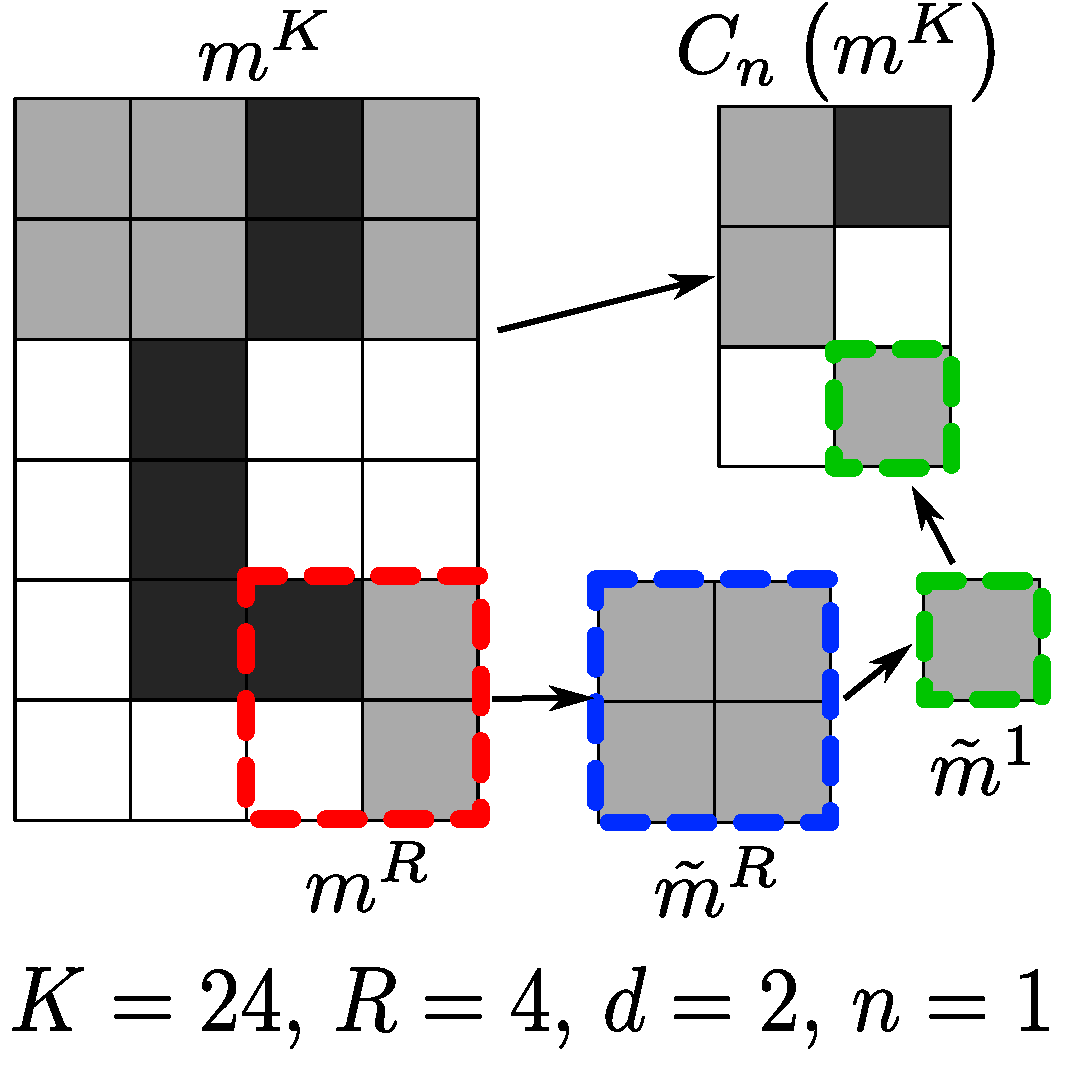
\includegraphics[height=5.8cm]{map_compression.pdf}
        \caption{Example OG compression sequence. \label{fig:pri_compression1}}
    \end{subfigure}
    \hfill
    \begin{subfigure}[t]{0.45\textwidth}
        \centering
        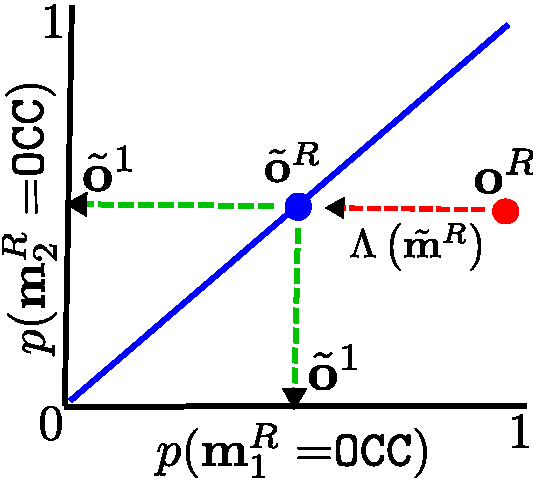
\includegraphics[height=5.8cm]{compression.pdf}
        \caption{Probability space of the top two grid cells
        in $\mbf{m}^{R}$ in~\ref{fig:pri_compression1}. \label{fig:pri_compression2}}
    \end{subfigure}
    \caption[Occupancy grid compression sequence.]{For each square (cubic in 3D)
      region $\mbf{m}^{R}$ in the uncompressed OG $\mbf{m}^{K}$,
      the PRI optimization finds a random variable $\tilde{\mbf{m}}^{R}$ that
    minimizes~\eqref{eq:pri_general} and is constrained to have uniform occupancy
    probability $\tilde{\mbf{o}}^{R} = (\tilde{\mbf{o}}^{1}, \dots,
    \tilde{\mbf{o}}^{1})$.
  \label{fig:pri_compression}}
\end{figure}

Using these notations alongside the PRI optimization in~\eqref{eq:pri_specific}, a
compressed OG region $\tilde{\mbf{m}}^{R}$ that minimizes entropy and divergence from
its uncompressed counterpart $\mbf{m}^{R}$ is that which maximizes $\Lambda(\tilde{\mbf{m}}^{R})$ in
%
\eq{
  \Lambda(\tilde{\mbf{m}}^{R})
  &=
  \max_{\tilde{\mbf{m}}^{R}}
  \sum_{\mc{M}^{R}}
  p(\mbf{m}^{R}) p(\tilde{\mbf{m}}^{R}),
}
%
Rather than finding the maximal value of the cost function itself, the
occupancy probability for the compressed OG region can be found by determining
$\tilde{\mbf{o}}^{1}$:
%
\eq{
  \tilde{\mbf{o}}^{1}_{*} &=
  \argmax_{\tilde{\mbf{o}}^{1}}
  \sum_{\mc{M}^{R}}
  p(\mbf{m}^{R}) p(\tilde{\mbf{m}}^{R}),
  \label{eq:pri_specific2}
}
%
In order to fully constrain the problem, it is important to note that
$p(\tilde{\mbf{m}}^{R})$ is a Bernoulli distribution. All of the cells in
$\tilde{\mbf{m}}^{R}$ have a uniform probability of occupancy and therefore
cannot differ from one another, as they must ultimately be compressed to a
scalar that represents the occupancy probability of a single cell. In other
words, $\tilde{\mbf{o}}^{1}$ is the probability of occupancy for every cell in
$\tilde{\mbf{m}}^{R}$.

\section{Solving the Optimization}
\label{sec:solving_pri}

Solving the optimization in~\eqref{eq:pri_specific2} involves iterating through all
permutations of maps that have cell count $R$ and multiplying the probability that
$\mbf{m}^{R}$ takes on a specific permutation with the probability that
$\tilde{\mbf{m}}^{R}$ takes on that permutation. Fortunately, although $\mc{M}^{R}$ is large
($\vert \mc{M}^{R} \vert = 2^{R}$), $p(\tilde{\mbf{m}}^{R})$ is zero for
all but two permutations due to the fact that $\tilde{\mbf{m}}^{R}$ must have
uniform occupancy. Specifically, the following is true:

\begin{itemize}
  \item
    $p(
    \tilde{\mbf{m}}^{R}
    \ne
    \{\texttt{EMP}, \dots, \texttt{EMP}\}
    \wedge
    \tilde{\mbf{m}}^{R}
    \ne
    \{\texttt{OCC}, \dots, \texttt{OCC}\}
    ) = 0$
  \item
    $p(\tilde{\mbf{m}}^{R}
    =
    \{\texttt{EMP}, \dots, \texttt{EMP}\}) = 1 - \tilde{\mbf{o}}^{R}$
  \item
    $p(\tilde{\mbf{m}}^{R}
    =
    \{\texttt{OCC}, \dots, \texttt{OCC}\}) = \tilde{\mbf{o}}^{R}$
  \item
    $p(\mbf{m}^{R} = \{\texttt{EMP},\dots,\texttt{EMP}\})
    =
    \prod_{i=1}^{R}(1-\mbf{o}^{R}_{i})$
  \item
    $p(\mbf{m}^{R} = \{\texttt{OCC},\dots,\texttt{OCC}\})
    =
    \prod_{i=1}^{R}\mbf{o}^{R}_{i}$
\end{itemize}

All map permutations in $\mc{M}^{R}$ for which $p(\tilde{\mbf{m}}^{R})$ is equal
to zero do not contribute to the sum in~\eqref{eq:pri_specific2}. The two
remaining non-zero terms in the summand of~\eqref{eq:pri_specific2} can be
enumerated explicitly:
%
\eq{
  \sum_{\mc{M}^{R}}
  p(\mbf{m}^{R}) p(\tilde{\mbf{m}}^{R})
  &=
  p(\mbf{m}^{R} = \{\texttt{EMP},\dots,\texttt{EMP}\})
  p(\tilde{\mbf{m}}^{R} = \{\texttt{EMP},\dots,\texttt{EMP}\})
  \\
  &\quad+
  p(\mbf{m}^{R} = \{\texttt{OCC},\dots,\texttt{OCC}\})
  p(\tilde{\mbf{m}}^{R} = \{\texttt{OCC},\dots,\texttt{OCC}\})
  \\
  &=
  (1 - \tilde{\mbf{o}}^{1})
  \prod_{i=1}^{R}
  (1 - \mbf{o}^{R}_{i})
  +
  \tilde{\mbf{o}}^{1}
  \prod_{i=1}^{R}
  \mbf{o}^{R}_{i}
  \label{eq:expanded_sum}
}
%
Substituting the expanded sum from~\eqref{eq:expanded_sum} into the optimization
from~\eqref{eq:pri_specific2}
gives
\eq{
  \tilde{\mbf{o}}_{*}^{1}
    &=
  \argmax_{\tilde{\mbf{o}}^{1}}
    \left(
    (1-\tilde{\mbf{o}}^{1}) \prod_{i=1}^{R}(1-\mbf{o}_{i}^{R})
    +\tilde{\mbf{o}}^{1} \prod_{i=1}^{R}\mbf{o}_{i}^{R}
    \right),
}
%
which is satisfied for
%
\eq{
  \tilde{\mbf{o}}_{*}^{1}
    &=
    \begin{cases}
      0           &\text{if} \ \prod_{i=1}^{R}\frac{\mbf{o}_{i}^{R}}{1-\mbf{o}_{i}^{R}} < 1 \\
      1           &\text{if} \ \prod_{i=1}^{R}\frac{\mbf{o}_{i}^{R}}{1-\mbf{o}_{i}^{R}} > 1 \\
    \frac{1}{2} &\text{otherwise}
    \end{cases},
    \label{eq:compression_cases}
}

where the last case is undefined for $\lambda=1$, but converges
to $\frac{1}{2}$ in the limit as $\lambda \rightarrow 1^{+}$.

The PRI OG compression solution yields a simple compression rule:
if the product of cell occupancy likelihoods in a given region is
greater than $1$, set the occupancy probability of the cell corresponding to
that region in the compressed OG to $1$. Likewise set the occupancy probability to $0$
if the product of likelihoods is less than $1$, and to $0.5$ if the
product of likelihoods is $1$.

Pragmatically, it is more reasonable to
use the map's occupancy and free thresholds rather than $1.0$ and $0.0$.
This variation corresponds to optimizing for $\lambda$ slightly greater
than one, favoring minimal distortion to minimal entropy. Additionally,
one may introduce a heuristic to increase the fraction of occupied cells
that are preserved through compression by multiplying the right-hand
sides of the inequalities in~\eqref{eq:compression_cases} by
$\eta \in (0, 1)$. As $\eta$ decreases, occupied cells will be preserved
through compression with higher frequency. For any application involving
raycasting, it is especially important to include this heuristic, as
vanishing occupied cells lead to poor ray termination.

Denoting $\pi^{R} \equiv
\prod_{i=1}^{R}\frac{\mbf{o}_{i}^{R}}{1-\mbf{o}_{i}^{R}}$ and applying
these modifications gives a rule for determining the occupancy probability of a
cell in the compressed map, given a $\sqrt{R}\times\sqrt{R}$ (in 2D) or
$\sqrt[3]{R}\times\sqrt[3]{R}\times\sqrt[3]{R}$ (in 3D) region $\mbf{m}^{R}$ of
the uncompressed
map:
%
\eq{
  \tilde{\mbf{o}}_{*}^{1}
    &=
    \begin{cases}
      \frac{1}{2}           &\text{if} \ \pi^{R} = \eta \vee \pi^{R} = 1 \\
    p_{\text{free}}         &\text{if} \ \pi^{R} < \eta \wedge \pi^{R} \ne 1 \\
    p_{\text{occ}}          &\text{if} \ \pi^{R} \ge \eta \wedge \pi^{R} \ne 1
    \end{cases},
    \label{eq:compression_cases2}
}
%
where $p_{\text{occ}}$ and $p_{\text{free}}$ are the thresholds for occupied and free space in the OG implementation, respectively.

\section{Occupancy Grid Pyramids}
\label{sec:og_pyramid}

In some situations it is useful to store multiple versions of the robot's map that are compressed
to different final resolutions. For example, Chapter~\ref{chapter4}
will compare maps of different resolutions to
investigate the amount of information lost about a sensor measurement through
compression. An \textit{occupancy grid pyramid} is a multi-resolution map data
structure that holds maps of several resolutions. This name is in reference to the image pyramid,
a multi-resolution image data structure used commonly in computer vision~\cite{adelson1984pyramid}.

To create an OG pyramid, one may simply apply increasing compressions to a base
OG. Each compressed map in the pyramid has $2^{-d}$ times as many
cells as the previous.
%
\eq{
  \mc{C}_{n}(\mbf{m}^{K})
  &\equiv
  \{
    \mbf{m}^{K},
    C_{1}(\mbf{m}^{K}),
    \dots,
    C_{n}(\mbf{m}^{K})
  \},
  \quad n \in \mbb{N}_{0}
}
%
All compressed maps are generated by applying $C_{n}$
(defined in~\eqref{eq:compression_definition})
to the base map, rather than by applying $C_{1}$ to the previous map in the
set. Depending on how one performs the compression, these may or may not result in
different pyramids.
A three-level OG pyramid is depicted in Fig.~\ref{fig:og_pyramid}.

\begin{figure}
  \centering
  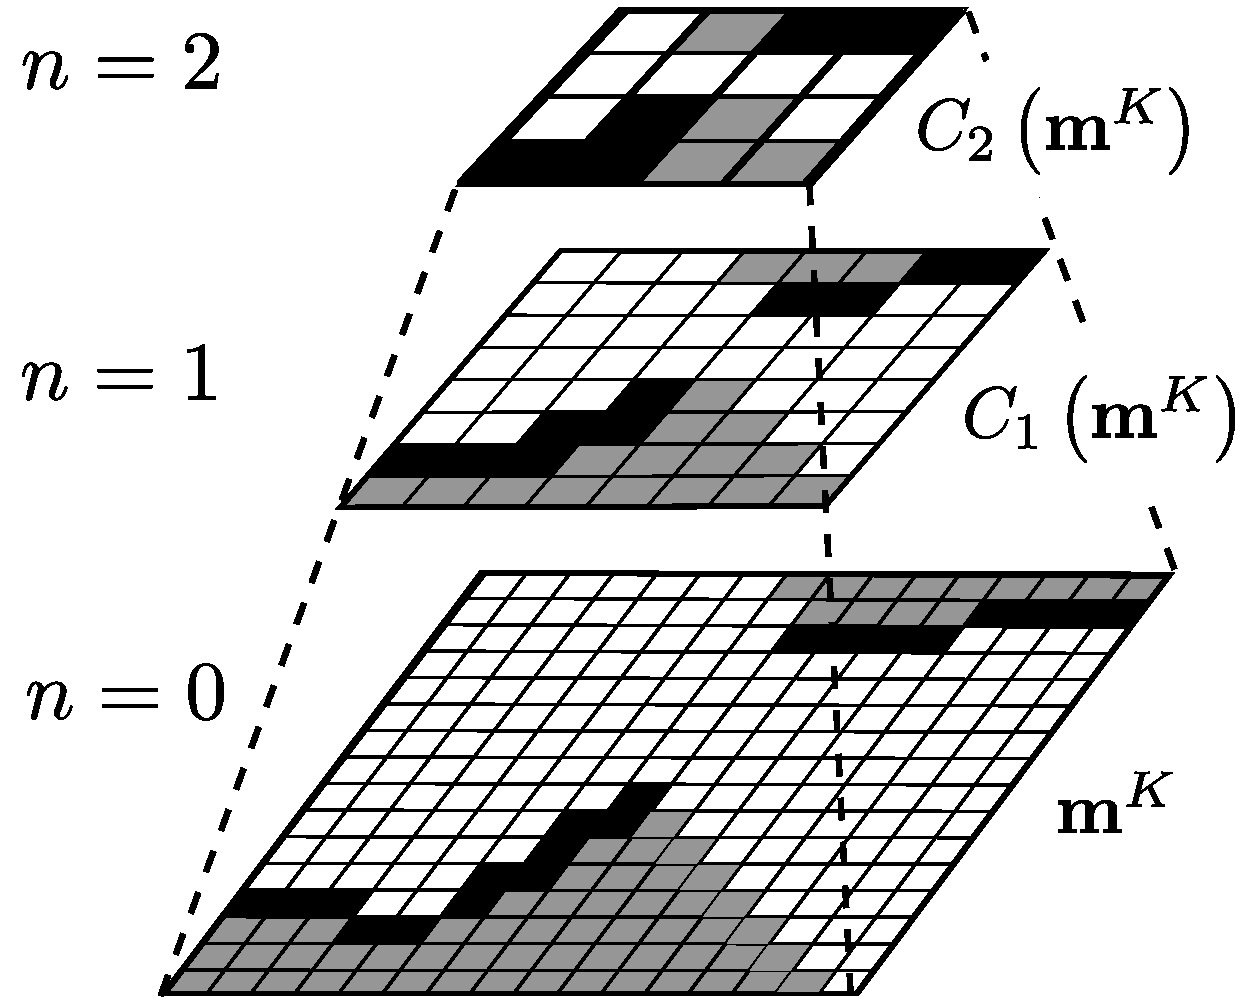
\includegraphics[width=0.4\textwidth]{pyramid.pdf}
  \caption[Diagram of a three-level OG pyramid.]{A three-level OG pyramid\label{fig:og_pyramid}}
\end{figure}

\section{Results}
\label{sec:chapter3_results}

Figure~\ref{fig:pri_result1} shows a six-level OG pyramid built by applying the PRI
optimization to a partially explored 2D map of a cluttered warehouse environment,
with $\eta = 0.2$. For values of
$\eta < 1$ the PRI compression strategy preserves and expands occupied cells in
the map, ensuring that raycasts that terminate on the uncompressed map will also
terminate on the compressed map. For $n=\{0,\dots,4\}$, intersections between
free and unknown space in the map is preserved. Several regions that are
occupied by obstacles in the uncompressed map are not represented well in
the map compressed with $n=5$.

\begin{figure}[H!]
  \centering
  \begin{subfigure}[t]{0.28\textwidth}
    \centering
    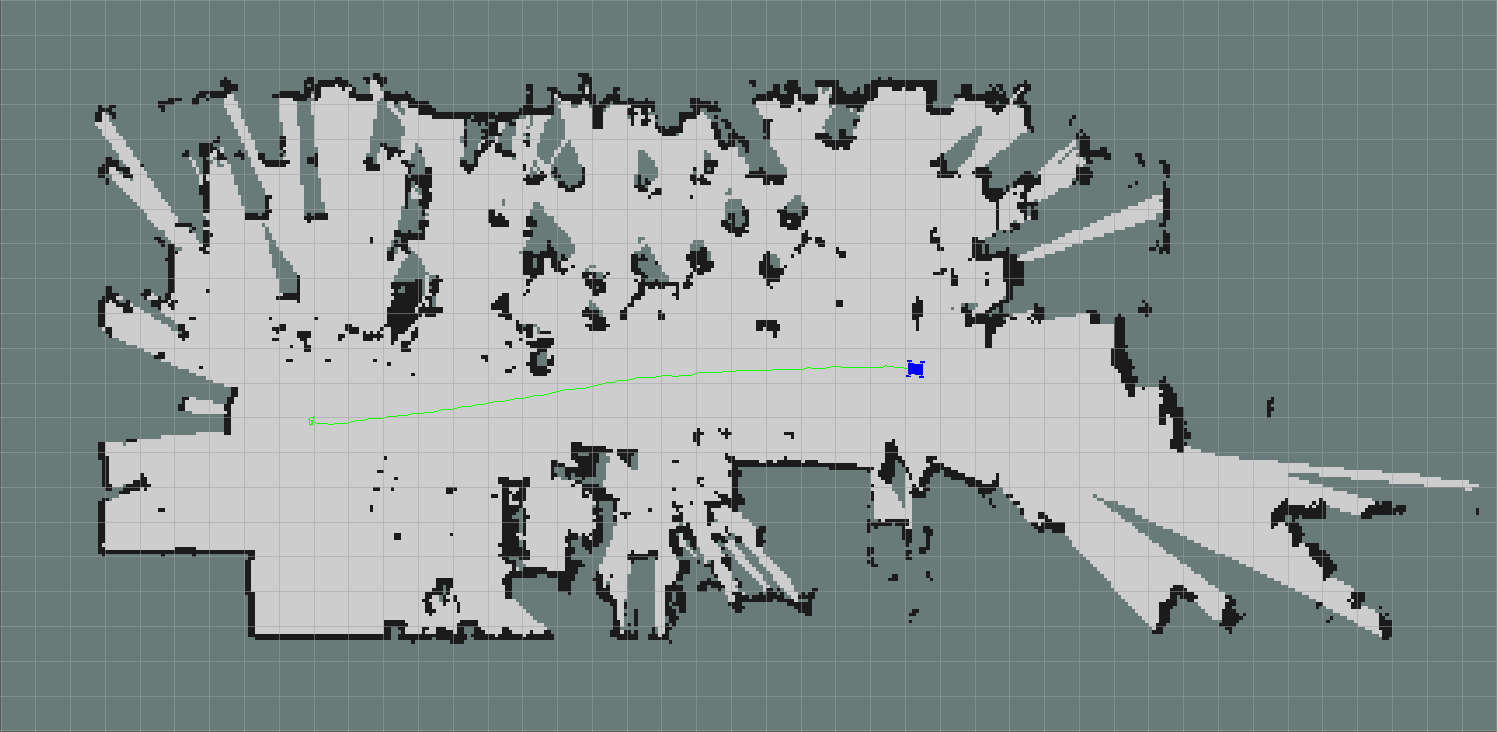
\includegraphics[angle=90, width=\textwidth]{compression0.png}
    \caption{$\mbf{m}$, $\Delta = 0.1$ m \label{fig:pri_result1_a}}
  \end{subfigure}
  \hfill
  \begin{subfigure}[t]{0.28\textwidth}
    \centering
    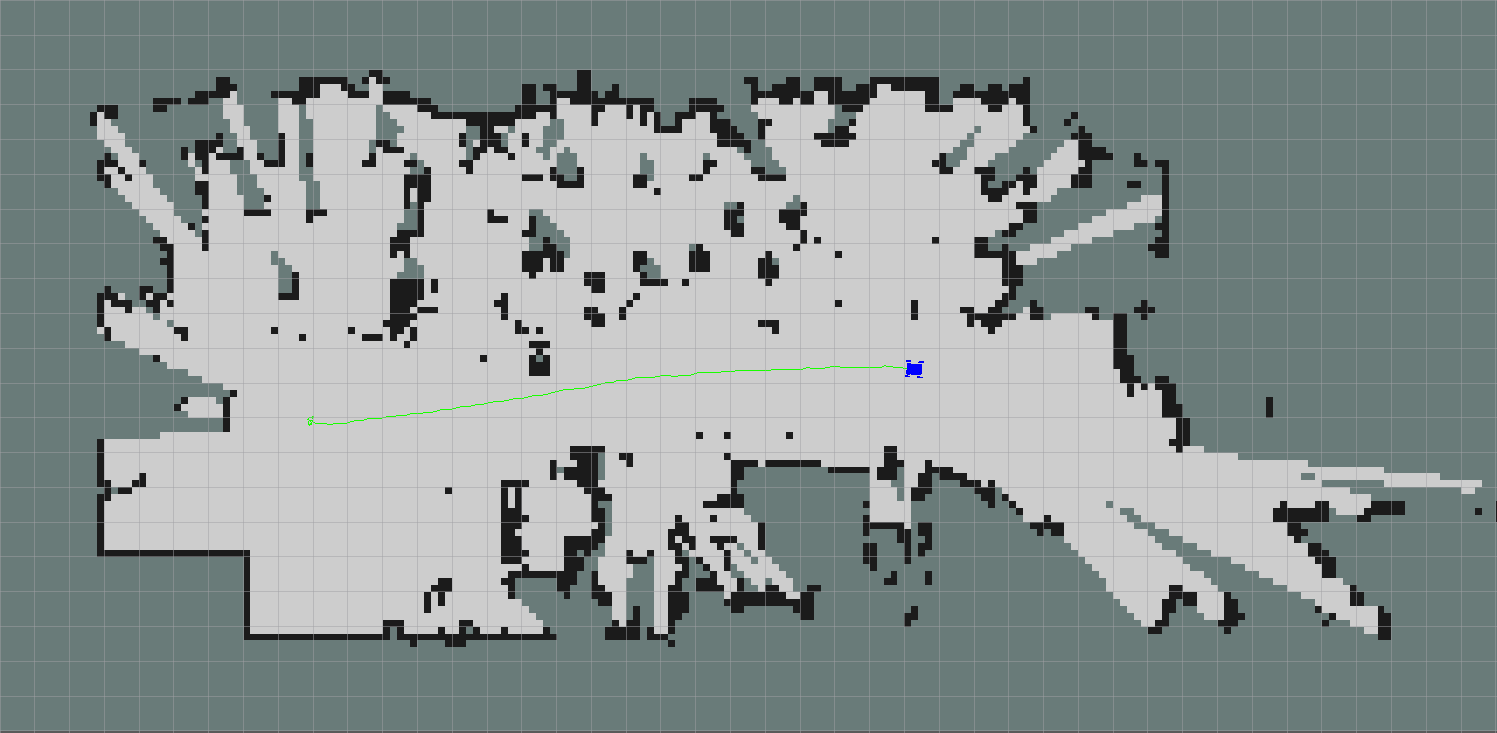
\includegraphics[angle=90, width=\textwidth]{compression1.png}
    \caption{$C_{1}(\mbf{m})$, $\Delta = 0.2$ m \label{fig:pri_result1_b}}
  \end{subfigure}
  \hfill
  \begin{subfigure}[t]{0.28\textwidth}
    \centering
    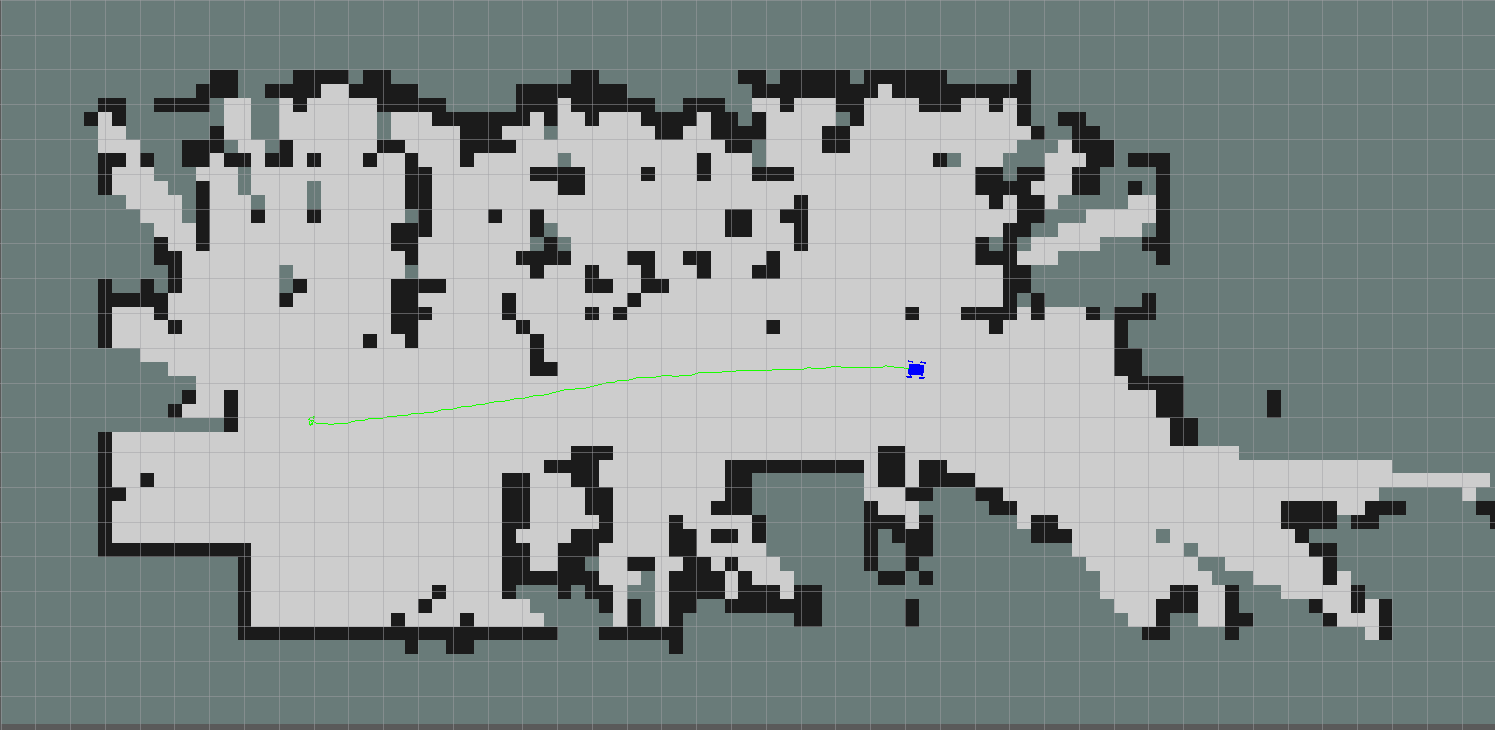
\includegraphics[angle=90, width=\textwidth]{compression2.png}
    \caption{$C_{2}(\mbf{m})$, $\Delta = 0.4$ m \label{fig:pri_result1_c}}
  \end{subfigure}
  \\
  \begin{subfigure}[t]{0.28\textwidth}
    \centering
    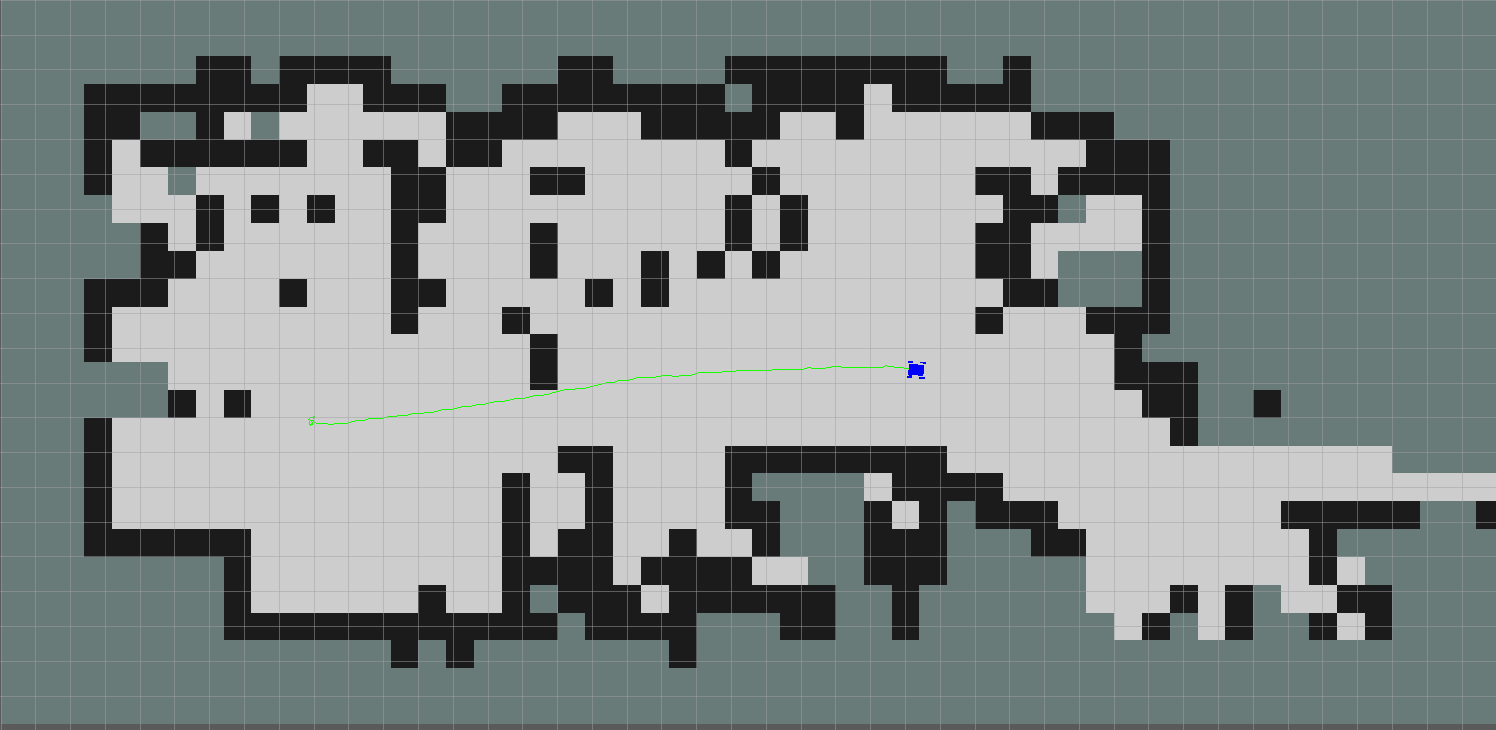
\includegraphics[angle=90, width=\textwidth]{compression3.png}
    \caption{$C_{3}(\mbf{m})$, $\Delta = 0.8$ m \label{fig:pri_result1_d}}
  \end{subfigure}
  \hfill
  \begin{subfigure}[t]{0.28\textwidth}
    \centering
    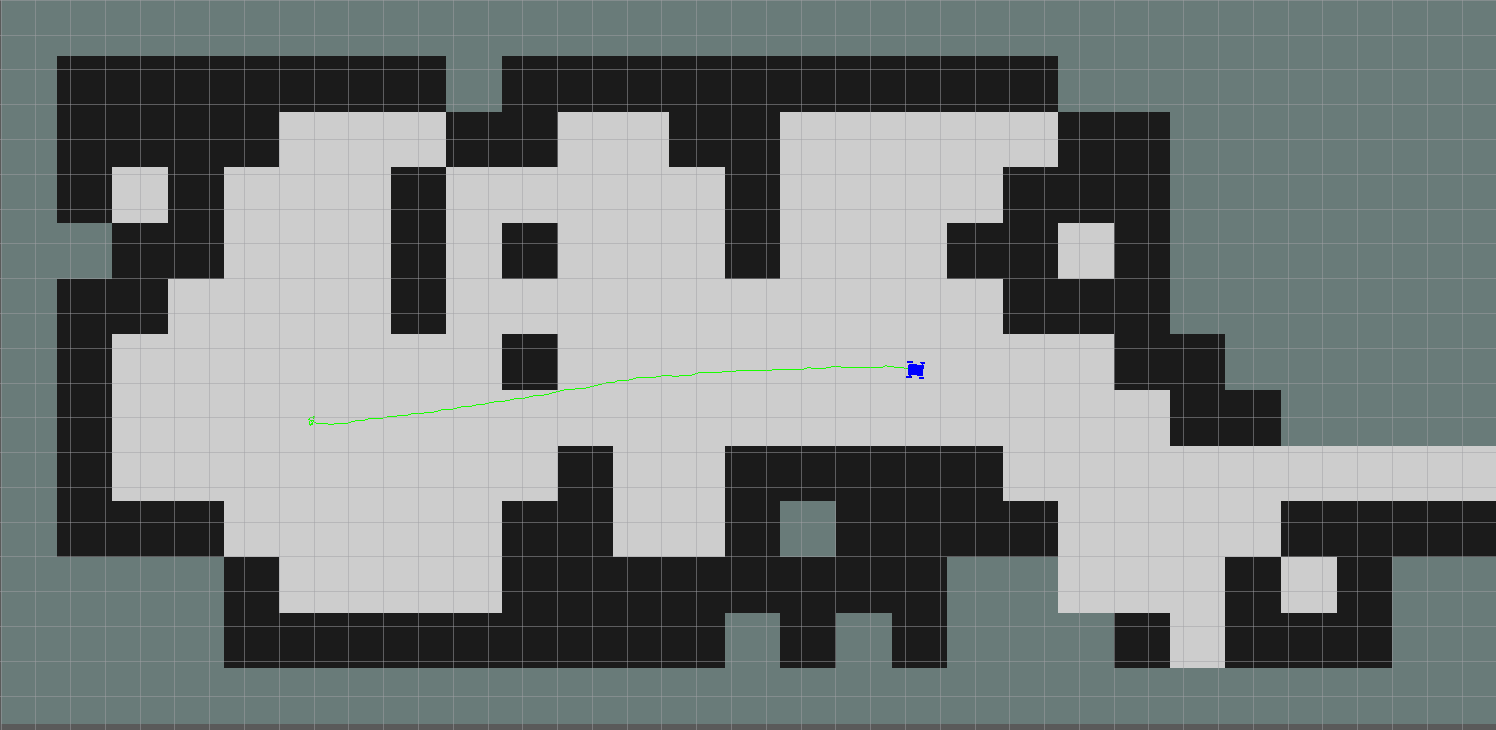
\includegraphics[angle=90, width=\textwidth]{compression4.png}
    \caption{$C_{4}(\mbf{m})$, $\Delta = 1.6$ m \label{fig:pri_result1_e}}
  \end{subfigure}
  \hfill
  \begin{subfigure}[t]{0.275\textwidth}
    \centering
    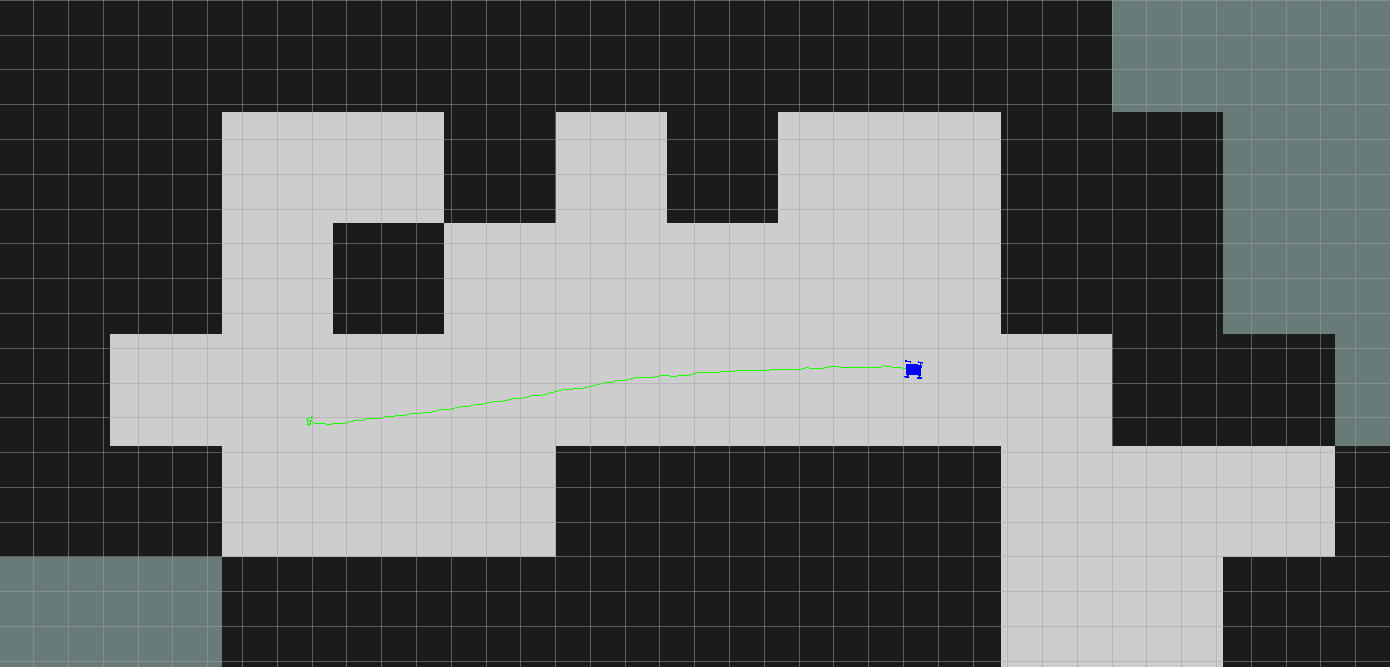
\includegraphics[angle=90, width=\textwidth]{compression5.png}
    \caption{$C_{5}(\mbf{m})$, $\Delta = 3.2$ m \label{fig:pri_result1_f}}
  \end{subfigure}
  \caption[A six-level OG pyramid built during exploration.]{A six-level OG pyramid $\mc{C}_{5}(\mbf{m})$, built from a
    partially explored 2D base OG, $\mbf{m}$, in a cluttered warehouse environment. The PRI compression strategy
    preserves boundaries between free and unknown space, and expands occupied cells.
  $\Delta$ denotes cell edge length. The robot is shown in blue, and its path in
  green.
\label{fig:pri_result1}}
\end{figure}

Map compression was motivated at the start of this chapter by the observation in
Fig.~\ref{fig:csqmi_timing} that compressing the map results in increased
efficiency of evaluating CSQMI. It is therefore important to ensure that
a sensor measurement that is informative to the uncompressed map is still
informative to a compressed map, and that map compression does not result in
major perturbations to the information value returned
by the CSQMI computation. Figure~\ref{fig:pri_result2} shows a library of
forward-arc motion primitives (Section~\ref{subsec:fa_motion_primitives})
planned from a simulated robot's current position into a partially explored map.
Reward is computed at the action endpoints using CSQMI between an expected future sensor
measurement and the compressed maps. High CSQMI reward actions have green
endpoints, while low CSQMI reward actions have red endpoints. The best action
according to the active perception optimization in~\eqref{eq:active_perception_csqmi} is shown
in blue. The relative rewards offered by actions retain their ordering until
the map is compressed significantly ($n=5$), at which point a different action
is chosen. Although different, the optimal action chosen for the map with
highest compression is still a high-reward path in the uncompressed
map. Computing CSQMI reward on the map with highest compression is $32$ times
more efficient than computing CSQMI reward using the uncompressed map.

\begin{figure}
  \centering
  \begin{subfigure}[t]{0.48\textwidth}
    \centering
    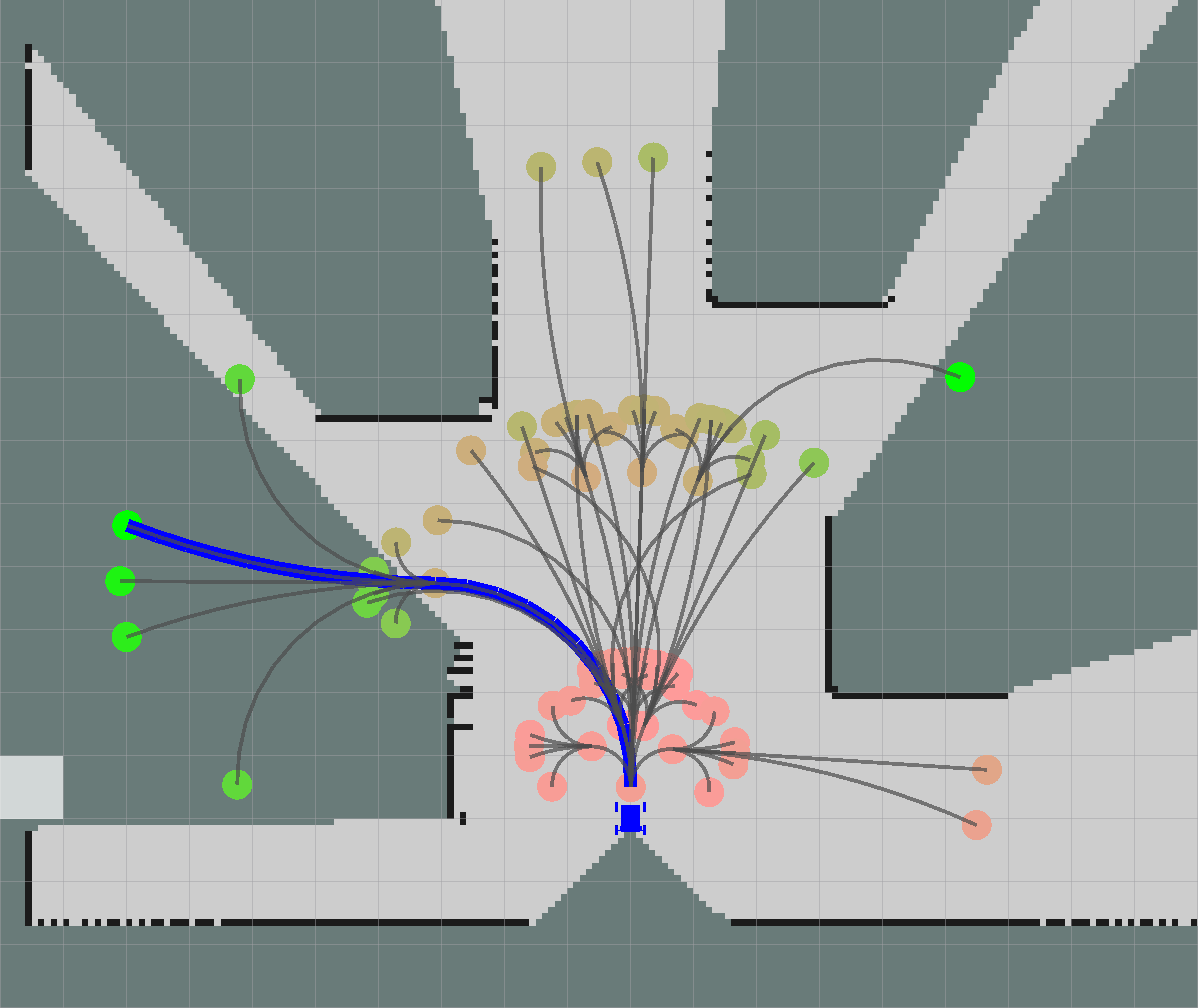
\includegraphics[width=\textwidth]{level0.png}
    \caption{$\mbf{m}$, $\Delta = 0.1$ m \label{fig:pri_result2_a}}
  \end{subfigure}
  \hfill
  \begin{subfigure}[t]{0.48\textwidth}
    \centering
    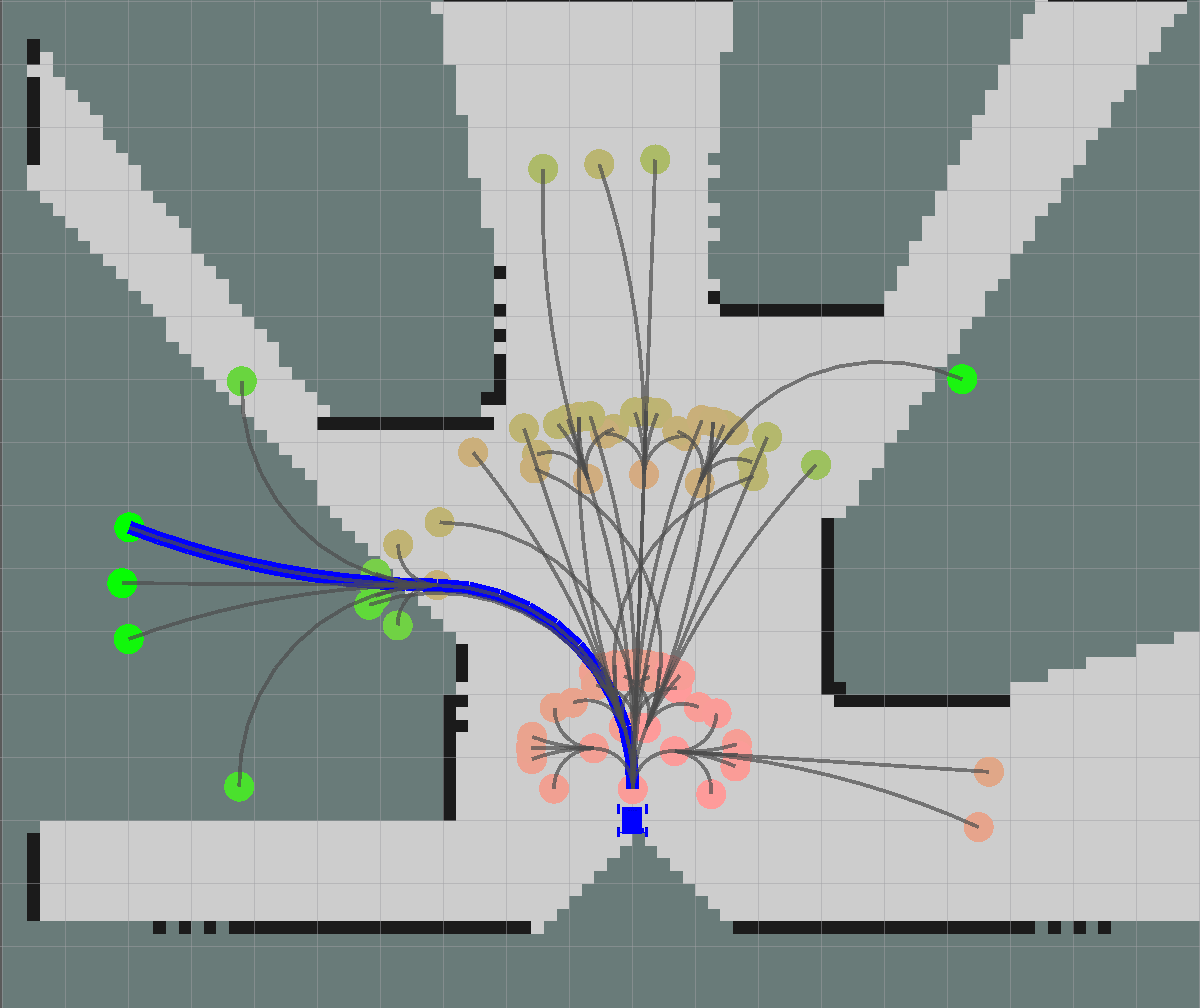
\includegraphics[width=\textwidth]{level1.png}
    \caption{$C_{1}(\mbf{m})$, $\Delta = 0.2$ m \label{fig:pri_result2_b}}
  \end{subfigure}
  \\
  \begin{subfigure}[t]{0.48\textwidth}
    \centering
    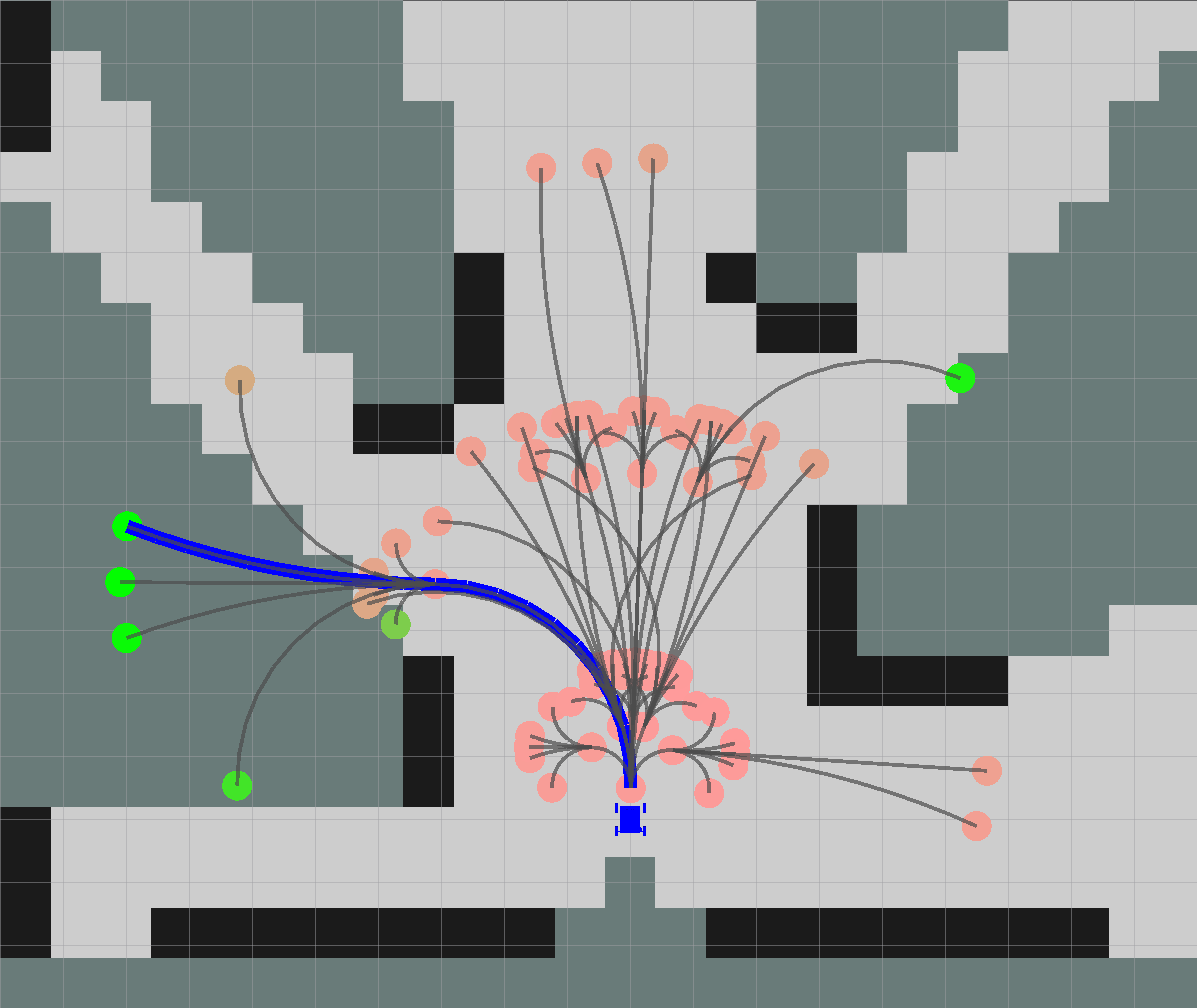
\includegraphics[width=\textwidth]{level3.png}
    \caption{$C_{3}(\mbf{m})$, $\Delta = 0.8$ m \label{fig:pri_result2_c}}
  \end{subfigure}
  \begin{subfigure}[t]{0.48\textwidth}
    \centering
    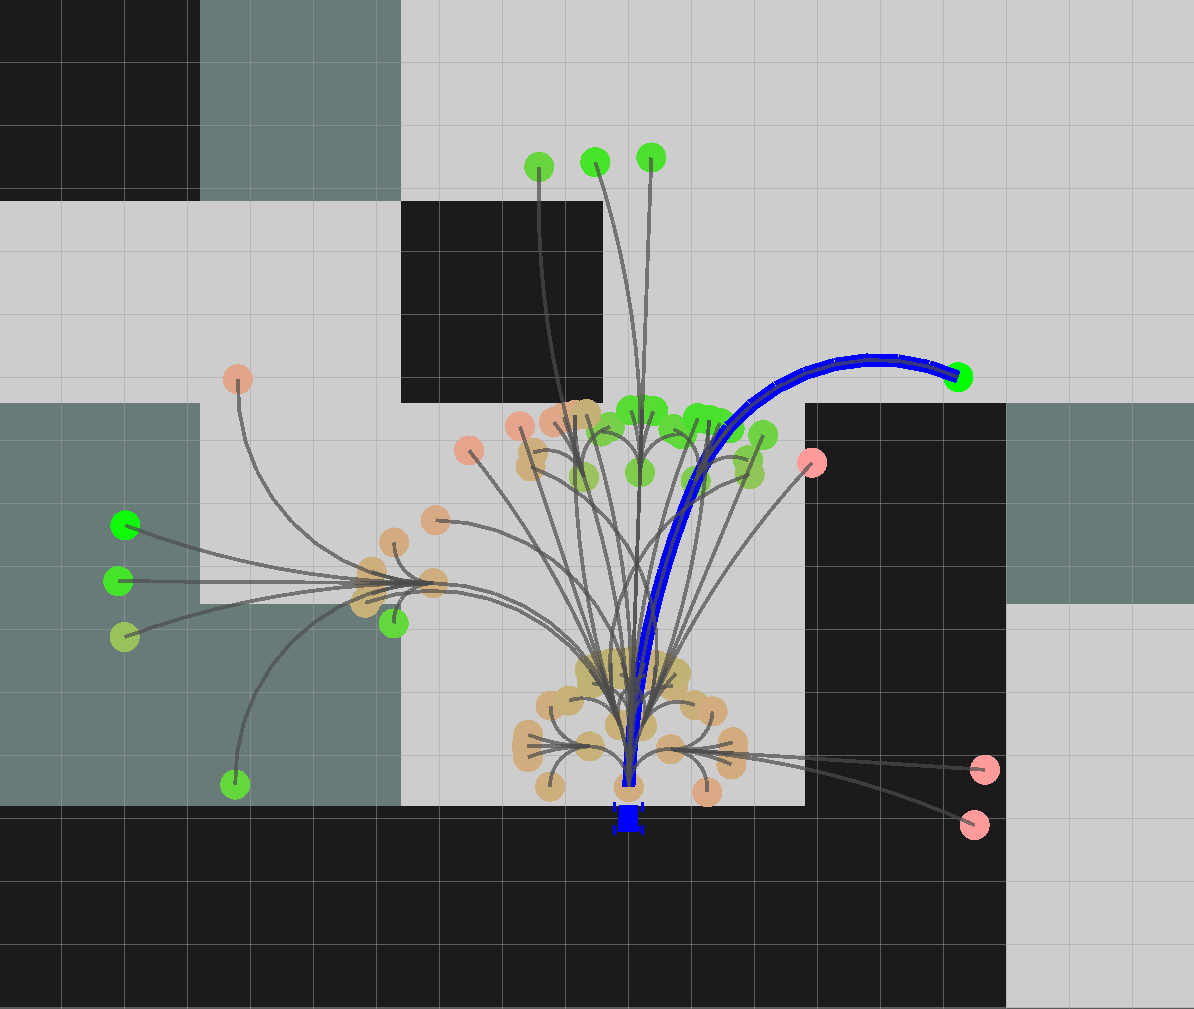
\includegraphics[width=\textwidth]{level5.png}
    \caption{$C_{5}(\mbf{m})$, $\Delta = 3.2$ m \label{fig:pri_result2_d}}
  \end{subfigure}
  \caption[Effects of map compression on CSQMI reward.]{The robot plans forward-arc motion primitives into a partially explored map with
    varying compression, calculating CSQMI reward at primitive endpoints. The optimal
    exploration action (blue) is not affected until a large ($n=5$) compression is
    applied. Green corresponds to high CSQMI reward, and red to low. $\Delta$
  denotes cell edge length. \label{fig:pri_result2}}
\end{figure}

Simulated exploration trials on a maze-like $25\times 25$ m map were
conducted to examine the effects of OG compression on a ground robot's exploration
path and planning frequency. To conduct these trials, a 2D dynamically constrained ground robot
equipped with a laser scanner and IMU was simulated. The robot was assumed to be
able to estimate its own state from incoming
sensor measurements and build an accurate OG of its surroundings in real-time.
To perform state estimation and mapping, the robot was outfitted with a laser-
and intertial-based SLAM implementation similar to that of Shen et
al.~\cite{shen2011autonomous}, leveraging ICP for laser odometry~\cite{pomerleau2013comparing},
a histogram filter for localization, and an
unscented Kalman filter (UKF) to fuse
estimates~\cite{thrun2005probabilistic}. A custom dense OG
implementation was used for mapping. The OG was updated at a
rate of $10$ Hz, and had a $0.1$ m/cell uncompressed resolution. The robot's
simulated laser scanner swept in a $270^{\circ}$ arc with $1081$ beams, and had
a max range of $30$ m.

In the simulated exploration trials, the map was compressed to a fixed
resolution ($n \in \{0, 2, 4\}$) using the PRI compression rule
in~\eqref{eq:compression_cases2}. The compressed OG was used to calculate CSQMI
along a set of planned actions. Resulting exploration paths are shown in
Fig.~\ref{fig:pri_result3}. To measure the increase in efficiency of computing
CSQMI reward from map compression, the number of actions output from the robot's
planner was increased until evaluating CSQMI reward at action endpoints
became prohibitevly expensive (roughly $1.5$ Hz planning frequency for a library
containing $81$ actions). Then, a goal velocity was chosen to make the robot
follow its highest-reward action without colliding with walls or reaching the end
of the action before a replan was triggered. With no map compression, this
resulted in a velocity of $0.35$ m/s, and the robot's total exploration time was
$230.0$ s.

The same exploration trial was run again,
calculating CSQMI reward with respect to compressed maps $C_{2}(\mbf{m})$ and $C_{4}(\mbf{m})$.
At $n=2$, the CSQMI reward for the $81$ actions could be evaluated at
approximately $6.0$ Hz, resulting in a safe navigation velocity of $1.50$ m/s
and a total exploration time of $54.7$ s.
At $n=4$, the CSQMI reward could be evaluated at $24.0$ Hz, yielding a velocity
of $3.00$ m/s and a total exploration time of $31.9$ s. Action collision checking
was performed with respect to a configuration space built from the uncompressed map
for all three trials. At $n=4$, a different action is chosen in the top-right corner
of the map, resulting in a different exploration path. The map is
mostly complete after each of the three trials. Numerical results from the
trials are shown in Table~\ref{tab:pri_result_table}.

\begin{figure}
    \centering
    \begin{subfigure}[t]{0.48\textwidth}
        \centering
        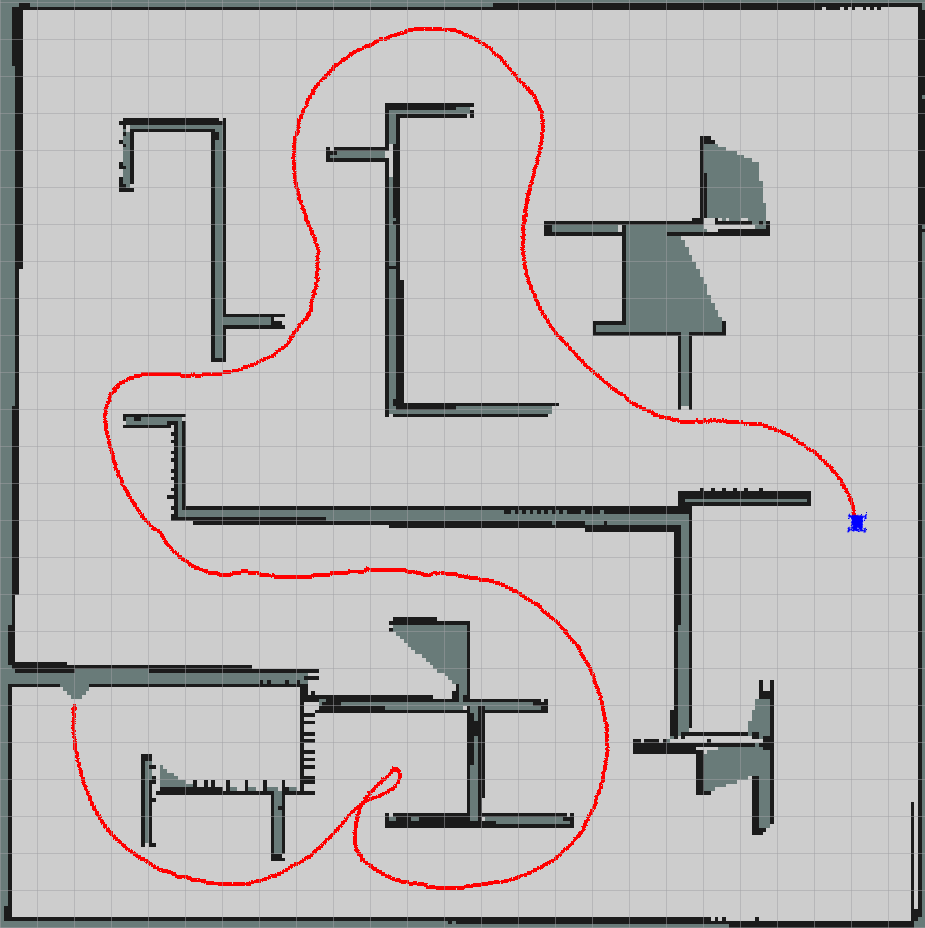
\includegraphics[width=\textwidth]{level0_explore_small.png}
        \caption{Velocity: $0.35$ m/s, no compression
        \label{fig:pri_result3_a}}
    \end{subfigure}
    \hfill
    \begin{subfigure}[t]{0.48\textwidth}
        \centering
        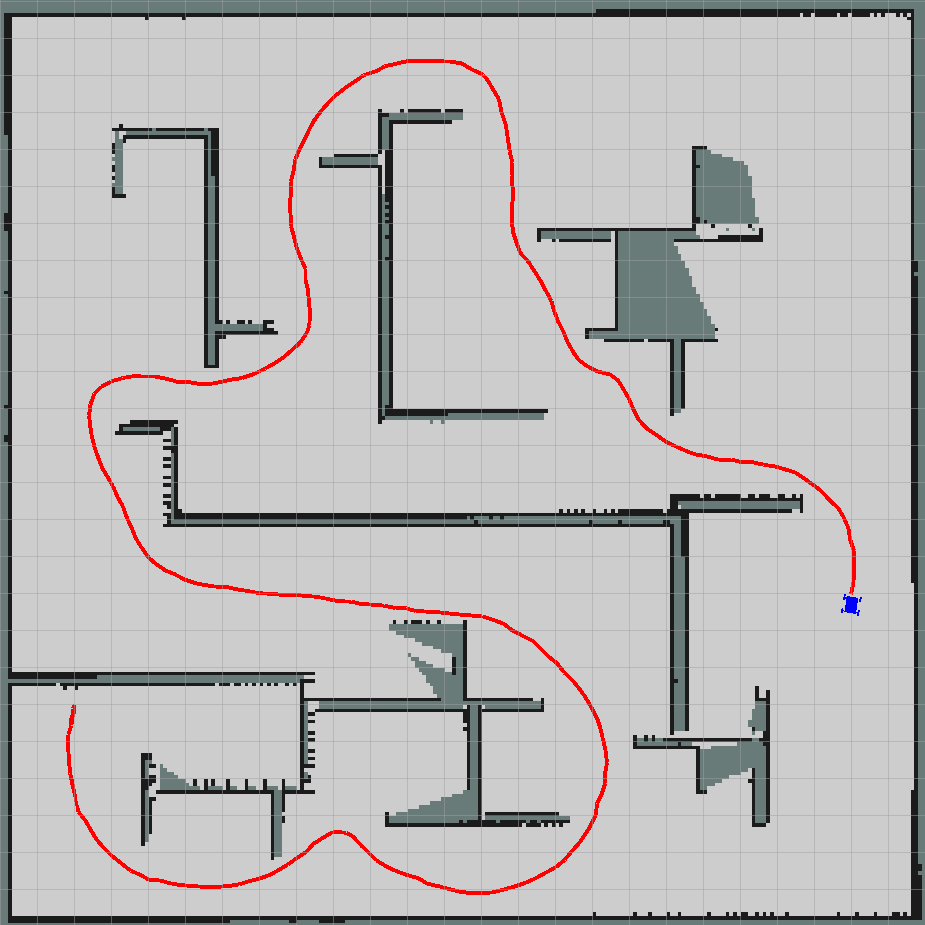
\includegraphics[width=\textwidth]{level2_explore_small.png}
        \caption{Velocity: $1.50$ m/s, $n=2$
        \label{fig:pri_result3_b}}
    \end{subfigure}
    \\
    \begin{subfigure}[t]{0.48\textwidth}
        \centering
        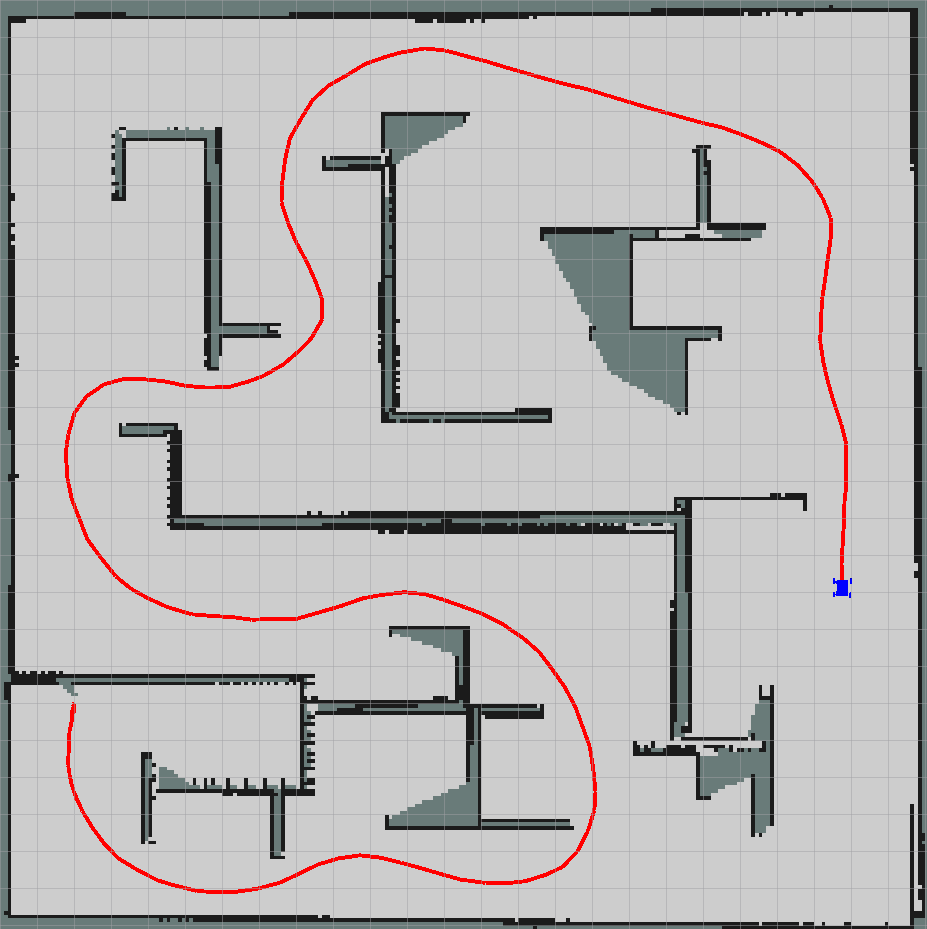
\includegraphics[width=\textwidth]{level4_explore_small.png}
        \caption{Velocity: $3.00$ m/s, $n=4$
        \label{fig:pri_result3_c}}
    \end{subfigure}
    \caption[Simulated exploration trials with map compression.]{Exploration paths when computing CSQMI with respect
    to: Fig.~\ref{fig:pri_result3_a} an uncompressed OG; Fig.~\ref{fig:pri_result3_b} an
OG compressed with $n=2$; Fig.~\ref{fig:pri_result3_c} an OG compressed with $n=4$.
Compressing the OG used for CSQMI computation leads to higher planning
frequencies, in turn enabling higher speed navigation. The uncompressed map is
shown in each figure to demonstrate completeness after exploration.
\label{fig:pri_result3}}
\end{figure}

\begin{table}[t]
  \caption[Simulated exploration trial results.]{Simulated exploration trial results
  (Fig.~\ref{fig:pri_result3}).\label{tab:pri_result_table}}
  \centering
  \begin{tabular}{| c | c | c | c | c |}
    \hline
    $n$ & {$\Delta$} (m) & Planning Freq. (Hz) &
            Maximum Velocity (m/s) & Time (s) \\ \hline
                                 0 & 0.1 & 1.5 & 0.35 & 230.0 \\ \hline
                                 2 & 0.4 & 6.0 & 1.50 & 54.7 \\ \hline
                                 4 & 1.6 & 24.0 & 3.00 & 31.9 \\ \hline
  \end{tabular}
\end{table}

\clearpage

\section{Chapter Summary}

Chapter~\ref{chapter3} formulated map compression as an information-theoretic
optimization using the Principle of Relevant Information. The optimization was
solved by decomposing an uncompressed OG into independent square (cubic in 3D) regions, and
compressing each region such that both its entropy and divergence with respect
to the uncompressed region were minimized. The PRI compression problem was solved lending equal
weight to minimum entropy and minimum divergence (i.e. $\lambda = 1$), which gave a simple
compression rule with three cases: a cell in the compressed OG can take on a
value of either $p_{\text{free}}$, $p_{\text{occ}}$, or $\frac{1}{2}$. The PRI compression strategy was applied to a
map of a large warehouse environment, and was shown to preserve boundaries
between free and unknown space, and to expand occupied cells for $\eta \in (0,
1)$.

Heuristics were introduced to avoid zero-valued or one-valued probabilities
in compressed OGs, and to ensure that occupied cells in
the uncompressed map are preserved through compression. Occupancy grid
pyramids were introduced as a mathematical tool for defining a set of OGs with
increasing compression.

Applying the PRI compression strategy to maps in a real cluttered warehouse
environment (Fig.~\ref{fig:pri_result1}), and in simulated maze environments
(Figs.~\ref{fig:pri_result2} and~\ref{fig:pri_result3}) allowed the robot to plan
actions more efficiently, which was hypothesized by Fig.~\ref{fig:csqmi_timing}.
Propagating the gains in planning efficiency through
to the robot's dynamics enabled the robot to explore faster when calculating
CSQMI reward with respect to a compressed map. After significant amounts of
compression, the robot began to select suboptimal exploration actions
(Figs.~\ref{fig:pri_result2_d} and~\ref{fig:pri_result3_c}). The distortion to
CSQMI reward with increasing map compression necessitates a
method for choosing a compression level in response to the robot's environment.

